%% bare_conf.tex
%% V1.3
%% 2007/01/11
%% by Michael Shell
%% See:
%% http://www.michaelshell.org/
%% for current contact information.
%%
%% This is a skeleton file demonstrating the use of IEEEtran.cls
%% (requires IEEEtran.cls version 1.7 or later) with an IEEE conference paper.
%%
%% Support sites:
%% http://www.michaelshell.org/tex/ieeetran/
%% http://www.ctan.org/tex-archive/macros/latex/contrib/IEEEtran/
%% and
%% http://www.ieee.org/

%%*************************************************************************
%% Legal Notice:
%% This code is offered as-is without any warranty either expressed or
%% implied; without even the implied warranty of MERCHANTABILITY or
%% FITNESS FOR A PARTICULAR PURPOSE! 
%% User assumes all risk.
%% In no event shall IEEE or any contributor to this code be liable for
%% any damages or losses, including, but not limited to, incidental,
%% consequential, or any other damages, resulting from the use or misuse
%% of any information contained here.
%%
%% All comments are the opinions of their respective authors and are not
%% necessarily endorsed by the IEEE.
%%
%% This work is distributed under the LaTeX Project Public License (LPPL)
%% ( http://www.latex-project.org/ ) version 1.3, and may be freely used,
%% distributed and modified. A copy of the LPPL, version 1.3, is included
%% in the base LaTeX documentation of all distributions of LaTeX released
%% 2003/12/01 or later.
%% Retain all contribution notices and credits.
%% ** Modified files should be clearly indicated as such, including  **
%% ** renaming them and changing author support contact information. **
%%
%% File list of work: IEEEtran.cls, IEEEtran_HOWTO.pdf, bare_adv.tex,
%%                    bare_conf.tex, bare_jrnl.tex, bare_jrnl_compsoc.tex
%%*************************************************************************

% *** Authors should verify (and, if needed, correct) their LaTeX system  ***
% *** with the testflow diagnostic prior to trusting their LaTeX platform ***
% *** with production work. IEEE's font choices can trigger bugs that do  ***
% *** not appear when using other class files.                            ***
% The testflow support page is at:
% http://www.michaelshell.org/tex/testflow/



% Note that the a4paper option is mainly intended so that authors in
% countries using A4 can easily print to A4 and see how their papers will
% look in print - the typesetting of the document will not typically be
% affected with changes in paper size (but the bottom and side margins will).
% Use the testflow package mentioned above to verify correct handling of
% both paper sizes by the user's LaTeX system.
%
% Also note that the "draftcls" or "draftclsnofoot", not "draft", option
% should be used if it is desired that the figures are to be displayed in
% draft mode.
%
\documentclass[a4paper]{IEEEtran}
\pagestyle{empty}

% Add the compsoc option for Computer Society conferences.
%
% If IEEEtran.cls has not been installed into the LaTeX system files,
% manually specify the path to it like:
% \documentclass[conference,a4paper]{../sty/IEEEtran}


% Some very useful LaTeX packages include:
% (uncomment the ones you want to load)

% *** MISC UTILITY PACKAGES ***
%
%\usepackage{ifpdf}
% Heiko Oberdiek's ifpdf.sty is very useful if you need conditional
% compilation based on whether the output is pdf or dvi.
% usage:
% \ifpdf
%   % pdf code
% \else
%   % dvi code
% \fi
% The latest version of ifpdf.sty can be obtained from:
% http://www.ctan.org/tex-archive/macros/latex/contrib/oberdiek/
% Also, note that IEEEtran.cls V1.7 and later provides a builtin
% \ifCLASSINFOpdf conditional that works the same way.
% When switching from latex to pdflatex and vice-versa, the compiler may
% have to be run twice to clear warning/error messages.


% *** CITATION PACKAGES ***
%
\usepackage{cite}
% cite.sty was written by Donald Arseneau
% V1.6 and later of IEEEtran pre-defines the format of the cite.sty package
% \cite{} output to follow that of IEEE. Loading the cite package will
% result in citation numbers being automatically sorted and properly
% "compressed/ranged". e.g., [1], [9], [2], [7], [5], [6] without using
% cite.sty will become [1], [2], [5]--[7], [9] using cite.sty. cite.sty's
% \cite will automatically add leading space, if needed. Use cite.sty's
% noadjust option (cite.sty V3.8 and later) if you want to turn this off.
% cite.sty is already installed on most LaTeX systems. Be sure and use
% version 4.0 (2003-05-27) and later if using hyperref.sty. cite.sty does
% not currently provide for hyperlinked citations.
% The latest version can be obtained at:
% http://www.ctan.org/tex-archive/macros/latex/contrib/cite/
% The documentation is contained in the cite.sty file itself.


% *** GRAPHICS RELATED PACKAGES ***
%
%\ifCLASSINFOpdf
  %\usepackage[pdftex]{graphicx}
  % declare the path(s) where your graphic files are
  % \graphicspath{{../pdf/}{../jpeg/}}
  % and their extensions so you won't have to specify these with
  % every instance of \includegraphics
  % \DeclareGraphicsExtensions{.pdf,.jpeg,.png}
%\else
  % or other class option (dvipsone, dvipdf, if not using dvips). graphicx
  % will default to the driver specified in the system graphics.cfg if no
  % driver is specified.
\usepackage[dvips]{graphicx}
  % declare the path(s) where your graphic files are
\graphicspath{{./}}
  % and their extensions so you won't have to specify these with
  % every instance of \includegraphics
\DeclareGraphicsExtensions{.eps}
%\fi
% graphicx was written by David Carlisle and Sebastian Rahtz. It is
% required if you want graphics, photos, etc. graphicx.sty is already
% installed on most LaTeX systems. The latest version and documentation can
% be obtained at: 
% http://www.ctan.org/tex-archive/macros/latex/required/graphics/
% Another good source of documentation is "Using Imported Graphics in
% LaTeX2e" by Keith Reckdahl which can be found as epslatex.ps or
% epslatex.pdf at: http://www.ctan.org/tex-archive/info/
%
% latex, and pdflatex in dvi mode, support graphics in encapsulated
% postscript (.eps) format. pdflatex in pdf mode supports graphics
% in .pdf, .jpeg, .png and .mps (metapost) formats. Users should ensure
% that all non-photo figures use a vector format (.eps, .pdf, .mps) and
% not a bitmapped formats (.jpeg, .png). IEEE frowns on bitmapped formats
% which can result in "jaggedy"/blurry rendering of lines and letters as
% well as large increases in file sizes.
%
% You can find documentation about the pdfTeX application at:
% http://www.tug.org/applications/pdftex

% *** MATH PACKAGES ***
%
\usepackage[cmex10]{amsmath}
\usepackage{amssymb}
% A popular package from the American Mathematical Society that provides
% many useful and powerful commands for dealing with mathematics. If using
% it, be sure to load this package with the cmex10 option to ensure that
% only type 1 fonts will utilized at all point sizes. Without this option,
% it is possible that some math symbols, particularly those within
% footnotes, will be rendered in bitmap form which will result in a
% document that can not be IEEE Xplore compliant!
%
% Also, note that the amsmath package sets \interdisplaylinepenalty to 10000
% thus preventing page breaks from occurring within multiline equations. Use:
%\interdisplaylinepenalty=2500
% after loading amsmath to restore such page breaks as IEEEtran.cls normally
% does. amsmath.sty is already installed on most LaTeX systems. The latest
% version and documentation can be obtained at:
% http://www.ctan.org/tex-archive/macros/latex/required/amslatex/math/


% *** SPECIALIZED LIST PACKAGES ***
%
%\usepackage{algorithmic}
% algorithmic.sty was written by Peter Williams and Rogerio Brito.
% This package provides an algorithmic environment fo describing algorithms.
% You can use the algorithmic environment in-text or within a figure
% environment to provide for a floating algorithm. Do NOT use the algorithm
% floating environment provided by algorithm.sty (by the same authors) or
% algorithm2e.sty (by Christophe Fiorio) as IEEE does not use dedicated
% algorithm float types and packages that provide these will not provide
% correct IEEE style captions. The latest version and documentation of
% algorithmic.sty can be obtained at:
% http://www.ctan.org/tex-archive/macros/latex/contrib/algorithms/
% There is also a support site at:
% http://algorithms.berlios.de/index.html
% Also of interest may be the (relatively newer and more customizable)
% algorithmicx.sty package by Szasz Janos:
% http://www.ctan.org/tex-archive/macros/latex/contrib/algorithmicx/


% *** ALIGNMENT PACKAGES ***
%
%\usepackage{array}
% Frank Mittelbach's and David Carlisle's array.sty patches and improves
% the standard LaTeX2e array and tabular environments to provide better
% appearance and additional user controls. As the default LaTeX2e table
% generation code is lacking to the point of almost being broken with
% respect to the quality of the end results, all users are strongly
% advised to use an enhanced (at the very least that provided by array.sty)
% set of table tools. array.sty is already installed on most systems. The
% latest version and documentation can be obtained at:
% http://www.ctan.org/tex-archive/macros/latex/required/tools/


%\usepackage{mdwmath}
%\usepackage{mdwtab}
% Also highly recommended is Mark Wooding's extremely powerful MDW tools,
% especially mdwmath.sty and mdwtab.sty which are used to format equations
% and tables, respectively. The MDWtools set is already installed on most
% LaTeX systems. The lastest version and documentation is available at:
% http://www.ctan.org/tex-archive/macros/latex/contrib/mdwtools/


% IEEEtran contains the IEEEeqnarray family of commands that can be used to
% generate multiline equations as well as matrices, tables, etc., of high
% quality.


%\usepackage{eqparbox}
% Also of notable interest is Scott Pakin's eqparbox package for creating
% (automatically sized) equal width boxes - aka "natural width parboxes".
% Available at:
% http://www.ctan.org/tex-archive/macros/latex/contrib/eqparbox/





% *** SUBFIGURE PACKAGES ***
%\usepackage[tight,footnotesize]{subfigure}
% subfigure.sty was written by Steven Douglas Cochran. This package makes it
% easy to put subfigures in your figures. e.g., "Figure 1a and 1b". For IEEE
% work, it is a good idea to load it with the tight package option to reduce
% the amount of white space around the subfigures. subfigure.sty is already
% installed on most LaTeX systems. The latest version and documentation can
% be obtained at:
% http://www.ctan.org/tex-archive/obsolete/macros/latex/contrib/subfigure/
% subfigure.sty has been superceeded by subfig.sty.


%\usepackage[caption=false]{caption}
%\usepackage[font=footnotesize]{subfig}
% subfig.sty, also written by Steven Douglas Cochran, is the modern
% replacement for subfigure.sty. However, subfig.sty requires and
% automatically loads Axel Sommerfeldt's caption.sty which will override
% IEEEtran.cls handling of captions and this will result in nonIEEE style
% figure/table captions. To prevent this problem, be sure and preload
% caption.sty with its "caption=false" package option. This is will preserve
% IEEEtran.cls handing of captions. Version 1.3 (2005/06/28) and later 
% (recommended due to many improvements over 1.2) of subfig.sty supports
% the caption=false option directly:
%\usepackage[caption=false,font=footnotesize]{subfig}
%
% The latest version and documentation can be obtained at:
% http://www.ctan.org/tex-archive/macros/latex/contrib/subfig/
% The latest version and documentation of caption.sty can be obtained at:
% http://www.ctan.org/tex-archive/macros/latex/contrib/caption/


% *** FLOAT PACKAGES ***
%
\usepackage{float}
%\usepackage{fixltx2e}
% fixltx2e, the successor to the earlier fix2col.sty, was written by
% Frank Mittelbach and David Carlisle. This package corrects a few problems
% in the LaTeX2e kernel, the most notable of which is that in current
% LaTeX2e releases, the ordering of single and double column floats is not
% guaranteed to be preserved. Thus, an unpatched LaTeX2e can allow a
% single column figure to be placed prior to an earlier double column
% figure. The latest version and documentation can be found at:
% http://www.ctan.org/tex-archive/macros/latex/base/



%\usepackage{stfloats}
% stfloats.sty was written by Sigitas Tolusis. This package gives LaTeX2e
% the ability to do double column floats at the bottom of the page as well
% as the top. (e.g., "\begin{figure*}[!b]" is not normally possible in
% LaTeX2e). It also provides a command:
%\fnbelowfloat
% to enable the placement of footnotes below bottom floats (the standard
% LaTeX2e kernel puts them above bottom floats). This is an invasive package
% which rewrites many portions of the LaTeX2e float routines. It may not work
% with other packages that modify the LaTeX2e float routines. The latest
% version and documentation can be obtained at:
% http://www.ctan.org/tex-archive/macros/latex/contrib/sttools/
% Documentation is contained in the stfloats.sty comments as well as in the
% presfull.pdf file. Do not use the stfloats baselinefloat ability as IEEE
% does not allow \baselineskip to stretch. Authors submitting work to the
% IEEE should note that IEEE rarely uses double column equations and
% that authors should try to avoid such use. Do not be tempted to use the
% cuted.sty or midfloat.sty packages (also by Sigitas Tolusis) as IEEE does
% not format its papers in such ways.





% *** PDF, URL AND HYPERLINK PACKAGES ***
%
\usepackage{url}
% url.sty was written by Donald Arseneau. It provides better support for
% handling and breaking URLs. url.sty is already installed on most LaTeX
% systems. The latest version can be obtained at:
% http://www.ctan.org/tex-archive/macros/latex/contrib/misc/
% Read the url.sty source comments for usage information. Basically,
% \url{my_url_here}.





% *** Do not adjust lengths that control margins, column widths, etc. ***
% *** Do not use packages that alter fonts (such as pslatex).         ***
% There should be no need to do such things with IEEEtran.cls V1.6 and later.
% (Unless specifically asked to do so by the journal or conference you plan
% to submit to, of course. )

\usepackage[top=2.4cm,left=1.5cm,right=1.5cm,bottom=3.5cm]{geometry}

% Set dimensions of columns, gap between columns, and paragraph indent
%\setlength{\textheight}{8.875in} \setlength{\textwidth}{6.875in}
\setlength{\columnsep}{0.24in} %\setlength{\topmargin}{0in}
%\setlength{\headheight}{0in} 
\setlength{\headsep}{0in}
\setlength{\parindent}{1.2pc}
%\setlength{\oddsidemargin}{-.1875in}  % Centers text.
%\setlength{\evensidemargin}{-.1875in}

% Add the period after section numbers.  Adjust spacing.
%\newcommand{\Section}[1]{\vspace{-8pt}\section{\hskip -1em.~~#1}\vspace{-3pt}}
%\newcommand{\SubSection}[1]{\vspace{-3pt}\subsection{\hskip -1em.~~#1}
 %       \vspace{-3pt}}
				
\begin{document}

%
% paper title
% can use linebreaks \\ within to get better formatting as desired
\title{Preparation of a Formatted Technical Work for \\ the ICEM\vspace{-.1em}}

\author{J. W. Haggle, \textit{Senior Member, IEEE}
	and L. L. Grigsby, \textit{Senior, IEEE}
\thanks{Financial support should be acknowledged here. Example: This work was supported in part by the U.S. Depart­ment of Com­merce under Grant BS123.}
\thanks{The paper title should be in uppercase and lowercase letters, not all uppercase.}
\thanks{The name and affiliation (including city and country) of each author must appear on the paper. Full names of authors are preferred in the author line, but are not required. Initials are used in the affiliation footnotes (see below). Put a space between authors' initials. Do not use all uppercase for authors' surnames.}
\thanks{Examples of affiliation footnotes:}% <-this % stops a space
\thanks{J. W. Hagge is with Nebraska Public Power, District Hastings, NE 68902 USA (e-mail: j.hagge@ieee.org).}% <-this % stops a space
\thanks{L. L. Grigsby is with the Department of Electrical Engineering, Auburn University, Auburn, AL 36849 USA (e-mail: l.grigsby@ieee.org)}% <-this % stops a space
\vspace{-.45em}
}

% make the title area
\maketitle

\thispagestyle{empty}
\begin{abstract}
This document is itself an example of the desired layout (inclusive of this abstract) and can be used as a template. 
 It contains information regarding desktop publishing format, type sizes, and typefaces. Style rules are provided that 
 explains how to handle equations, units, figures, tables, abbreviations, and acronyms. Sections are also devoted to the 
 preparation of acknowledgments, references, and authors' biographies. The abstract is limited to 150 words and cannot 
 contain equations, figures, tables, abbreviations or references. It should concisely state what was done, how it was done,
 principal results, and their significance.
\end{abstract}

\vspace{1em}

\begin{IEEEkeywords}
The author shall provide up to 10 keywords (in alphabetical order) to help identify the major topics of the paper and to be enough referenced. The thesaurus of IEEE indexing keywords should be referenced prior to selecting the keywords to ensure that the words selected are acceptable. 
The thesaurus is posted at: 

\url{http://www.ieee.org/documents/2009Taxonomy_v101.pdf}
\end{IEEEkeywords}

% IEEEtran.cls defaults to using nonbold math in the Abstract.
% This preserves the distinction between vectors and scalars. However,
% if the conference you are submitting to favors bold math in the abstract,
% then you can use LaTeX's standard command \boldmath at the very start
% of the abstract to achieve this. Many IEEE journals/conferences frown on
% math in the abstract anyway.


% For peer review papers, you can put extra information on the cover
% page as needed:
% \ifCLASSOPTIONpeerreview
% \begin{center} \bfseries EDICS Category: 3-BBND \end{center}
% \fi
%
% For peerreview papers, this IEEEtran command inserts a page break and
% creates the second title. It will be ignored for other modes.
%\IEEEpeerreviewmaketitle

\section{Nomenclature}
A nomenclature list, if needed, should precede the Introduction.

\section{Introduction}
This document provides an example of the desired layout for a published ICEM technical work and can be used as a Microsoft Word template. 
It contains information regarding desktop publishing format, type sizes, and typefaces. Style rules are provided that explain how to handle equations, units, 
figures, tables, abbreviations, and acronyms. Sections are also devoted to the preparation of acknowledgments, references, and authors’ biographies.
\section{Technical Work Preparation}
Please use automatic hyphenation and check your spelling. Additionally, be sure your sentences are complete and that there is continuity within your paragraphs. 
Check the numbering of your graphics (figures and tables) and make sure that all appropriate references are included.
\subsection{Template}                  
This document may be used as a template for preparing your Transactions paper. You may type over sections of the document,
cut and paste into it, and/or use markup styles.
\subsection{Format}
If you choose not to use this document as a template, prepare your technical work in single-spaced, double-column format, on paper A4 (21x29.7 centimeters). 
Set top and bottom margins to 17 millimeters and left and right margins to about 17 millimeters. Do not violate margins 
(i.e., text, tables, figures, and equations may not extend into the margins). 
The column width is 85 millimeters. The space between the two columns is 5 millimeters. Paragraph indentation is 6 millimeters. Use full justification. 
Use either one or two spaces between sections, and between text and tables or figures, to adjust the column length.
\subsection{Typefaces and Sizes}
Please use a proportional serif typeface such as Times Roman or Times New Roman and embed all fonts. (See your software’s “Help” section if you do not know how to embed fonts.) 
Table I provides samples of the appropriate type sizes and styles to use.
%
\begin{table}[H]
\caption{Samples of Times Roman Type Sizes and Styles Used for Formatting a ICEM  Technical Work.\label{tab:Comparison-of-pattern}}
%\begin{centering}
\begin{figure}[H]
\begin{centering}
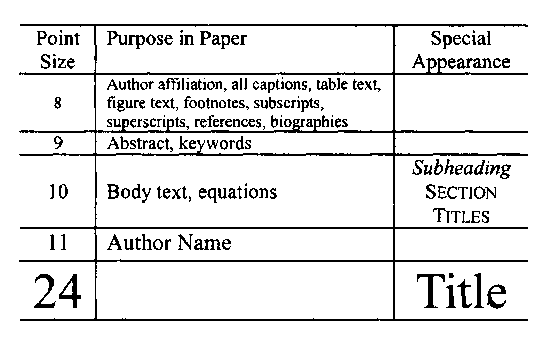
\includegraphics[scale=.9]{img2}
\par\end{centering}
\end{figure}

% \begin{tabular}{|c|c|c|}
% \cline{2-3} 
% \multicolumn{1}{c|}{} & A & B\tabularnewline
% \hline 
% row & $x$ & $y$\tabularnewline
% \hline 
% column & $1+x$ & $y-1$\tabularnewline
% \hline
%\end{tabular}
%\par\end{centering}

\end{table}

\subsection{Section Headings}
A primary section heading is enumerated by a Roman numeral followed by a period and is centered above the text. A primary heading should be in capital letters.
A secondary section heading is enumerated by a capital letter followed by a period and is flush left above the section. The first letter of each important word is capitalized and the heading is italicized.
A tertiary section heading is enumerated by an Arabic numeral followed by a parenthesis. It is indented and is followed by a colon. The first letter of each important word is capitalized and the heading is italicized.
A quaternary section heading is rarely necessary, but is perfectly acceptable if required. It is enumerated by a lowercase letter followed by a parenthesis. It is indented and is followed by a colon. Only the first letter of the heading is capitalized and the heading is italicized.
\subsection{Figures and Tables}
Figure axis labels are often a source of confusion. Try to use words rather than symbols. As an example, write the quantity "Magnetization," or "Magnetization, M," not just "M." Put units in parentheses. Do not label axes only with units. As in Fig. 1, write "Magnetization (kA/m)" or "Magnetization (kA·m-1)," not just "kA/m." Do not label axes with a ratio of quantities and units. For example, write "Temperature (K)," not "Temperature/K." Figure labels should be legible, approximately 8- to 10-point type.
Large figures and tables may span both columns, but may not extend into the page margins. Figure captions should be below the figures; table captions should be above the tables. Do not put captions in "text boxes" linked to the figures. Do not put borders around your figures.
All figures and tables must be in place in the text near, but not before, where they are first mentioned. Use the abbreviation "Fig. 1," even at the beginning of a sentence.
Digitize your tables and figures. To insert images in Word, use Insert | Picture | From File.

\begin{figure}[H]
\begin{centering}
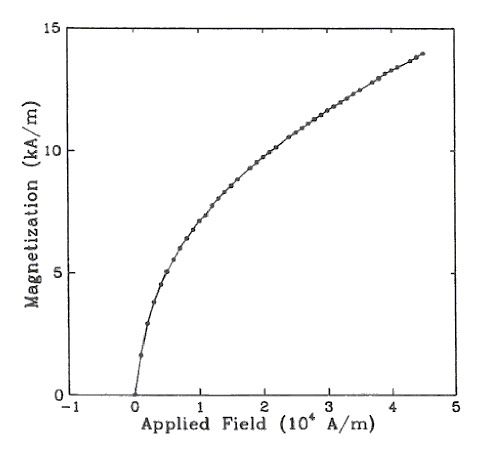
\includegraphics[scale=1]{img}
\par\end{centering}

\caption{Magnetization as a function of applied field. (Note that "Fig." is abbreviated and there is a period after the figure number followed by two spaces.).\label{img}}

\end{figure}

\subsection{Numbering}
Number reference citations consecutively in square brackets [1]. The sentence punctuation follows the brackets [2]. Multiple references [2], [3] are each numbered with separate brackets [1]-[3]. Refer simply to the reference number, as in [3]. Do not use "Ref. [3]" or "reference [3]" except at the beginning of a sentence: "Reference [3] shows….".
Number footnotes separately with superscripts (Insert | Footnote). Place the actual footnote at the bottom of the column in which it is cited. Do not put footnotes in the reference list. Use letters for table footnotes.
Check that all figures and tables are numbered correctly. Use Arabic numerals for figures and Roman numerals for tables.
Appendix figures and tables should be numbered consecutively with the figures and tables appearing in the rest of the paper. They should not have their own numbering system.
\subsection{Units}
Metric units are preferred in light of their global readership and the inherent convenience of these units in many fields. In particular, the use of the International System of Units (“Système International d'Unités” or SI Units) is advocated. This system includes a subsystem of units based on the meter, kilogram, second, and ampere (MKSA). British units may be used as secondary units (in parentheses). An exception is when British units are used as identifiers in trade, such as 3.5-inch disk drive.
\subsection{Abbreviations and Acronyms }
Define less common abbreviations and acronyms the first time they are used in the text (starting in the introduction and not before). Abbreviations such as IEEE, SI, MKS, CGS, AC, DC, and rms do not have to be defined. Do not use abbreviations in the title.
\subsection{Math and Equations}
Use either the Microsoft Equation Editor or the MathType commercial add-on for MS Word for all math objects in your paper (Insert | Object | Create New | Microsoft Equation or MathType Equation). "Float over text" should not be selected.
To make your equations more compact, you may use the solidus ( / ), the exp function, or appropriate exponents. Italicize Roman symbols for quantities and variables, but not Greek symbols. Use a long dash rather than a hyphen for a minus sign. Use parentheses to avoid ambiguities in denominators.
Number equations consecutively with equation numbers in parentheses flush with the right margin, as in (1). Be sure that the symbols in your equation have been defined before the equation appears or immediately following.
\begin{equation}
I_F = I_B = -I_C = A^{2}I_{A1}+AI_{A2}+I_{A0}=\frac{-J \sqrt{3}E_A}{Z_1+Z_2}
\end{equation}
\section{Appendix}
Appendixes, if needed, appear before the acknowledgment. 
\section{Acknowledgment}
The following is an example of an acknowledgment. Please note that financial support should be acknowledged in the unnumbered footnote on the title page.
The authors gratefully acknowledge the contributions of I.X. Austan, A.H. Burgmeyer, C.J. Essel, and S.H. Gold for their work on the original version of this document.
\section{References}
References are important to the reader. Therefore, each citation must be complete and correct. There is no editorial check on references. An incomplete or wrong reference will be published unless caught by a reviewer and will detract from the authority and value of the paper. References should be readily available publications.
List only one reference per reference number. If a reference is available from two sources, each should be listed as a separate reference. Give all authors' names; do not use et al. 
Samples of the correct formats for various types of references are given below (please do give only what is available at the international level with database or web accesses). References in languages other than English are strongly discouraged.

\cite{bishop_neural_1995}
\cite{mas_application_2008}
\cite{melin_hybrid_2005}
\cite{kavzoglu_increasing_2009}
\cite{agatonovic-kustrin_basic_2000}

\bibliographystyle{IEEEtran}
\bibliography{MyLibrary}

\section{Biographies}
A technical biography for each author must be included. It should begin with the author’s name (as it appears in the byline). Please do try to finish the two last columns on the last page at the same height. The following is an example of the text of a technical biography:
\begin{IEEEbiographynophoto}{Nikola Tesla}
 was born in Smiljan in the Austro-Hungarian Empire, on July 9, 1856. He graduated from the Austrian Polytechnic School, Graz, and studied at the University of Prague.
His employment experience included the American Telephone Company, Budapest, the Edison Machine Works, Westinghouse Electric Company, and Nikola Tesla Laboratories. His special fields of interest included high frequency.
Tesla received honorary degrees from institutions of higher learning including Columbia University, Yale University, University of Belgrade, and the University of Zagreb. He received the Elliott Cresson Medal of the Franklin Institute and the Edison Medal of the IEEE. In 1956, the term "Tesla" (T) was adopted as the unit of magnetic flux density in the MKSA system. In 1975, the Power Engineering Society established the Nikola Tesla Award in his honor. Tesla died on January 7, 1943.J. John
\end{IEEEbiographynophoto}

\end{document}
